\chapter{Design Analysis}
\label{ch:Design Analysis}



YOOOOOOO WAGWAN THIS IS SOME COOL PLACEHOLDER TEXT

\textcolor{blue}{I LOOOOOOVVVEEE it!! \\
    -The Burger King (Louisville, Kentucky 1407)\\
        -King Arthur (Came a lot, some castle 200 b.c.)\\
            -Cleopatra (Middle Earth, On a T-Rex 64 Million B.C.)\\
                -Batman (some rich kids school, right after his parents died)}
\section{Assumptions made for stiffness calculations}
The loading of the wingbox has been determined, and now the deflections can be calculated to find the structural and geometric requirements. The process for this can get quite complex, which is why some  assumptions will be made to simplify the calculations:
    To test the rigidity of the wing structure some simplifications needed to be made to properly be able to test it.
\begin{description}
    \item[Only wingbox is subject to loads] This assumption is a conservative estimate, as part of the loads will be distributed onto the skin, thus, it will result in a stronger stringer than strictly necessary for the full loading described in \autoref{ch:ForceDiagram}.
    
    \item[Constant thickness throughout a plate] This can be done because most commercial plates have a singular thickness and choosing a thickness for every span position, would overcomplicate making the tool.

    \item[Spar position is constant relative to chord length] This assumption allows the height of the spars to be linearly scaled with the chord. This will simplify the moment of inertia calculations for each spanwise point.

    \item[Stringer position in constant relative to chord length] This assumption will make sure that the stingers can always be spaced in a way to prevent buckling. This way only the worst case of spacing needs to be considered.

    \item[All panels are a single part with no cuts i.e. no 2 panels fastened] This assumption will allow for the use of the equations provided by the reader, without having to consider points with higher stress concentrations \cite{Timmer2024Project5}.
\end{description}
    
\section{Method}
% To produce designs that met the required specifications, the procedure shown in \autoref{fig:sketch_designs_procedure} was followed. This process needed to be repeated for all the possible combinations of the parameters that are being analyzed. The designs that meet the requirements will later be compared. The final choice will be made based on the mass of the design and the design philosophies.

% \begin{figure}[H]
%     \centering
%     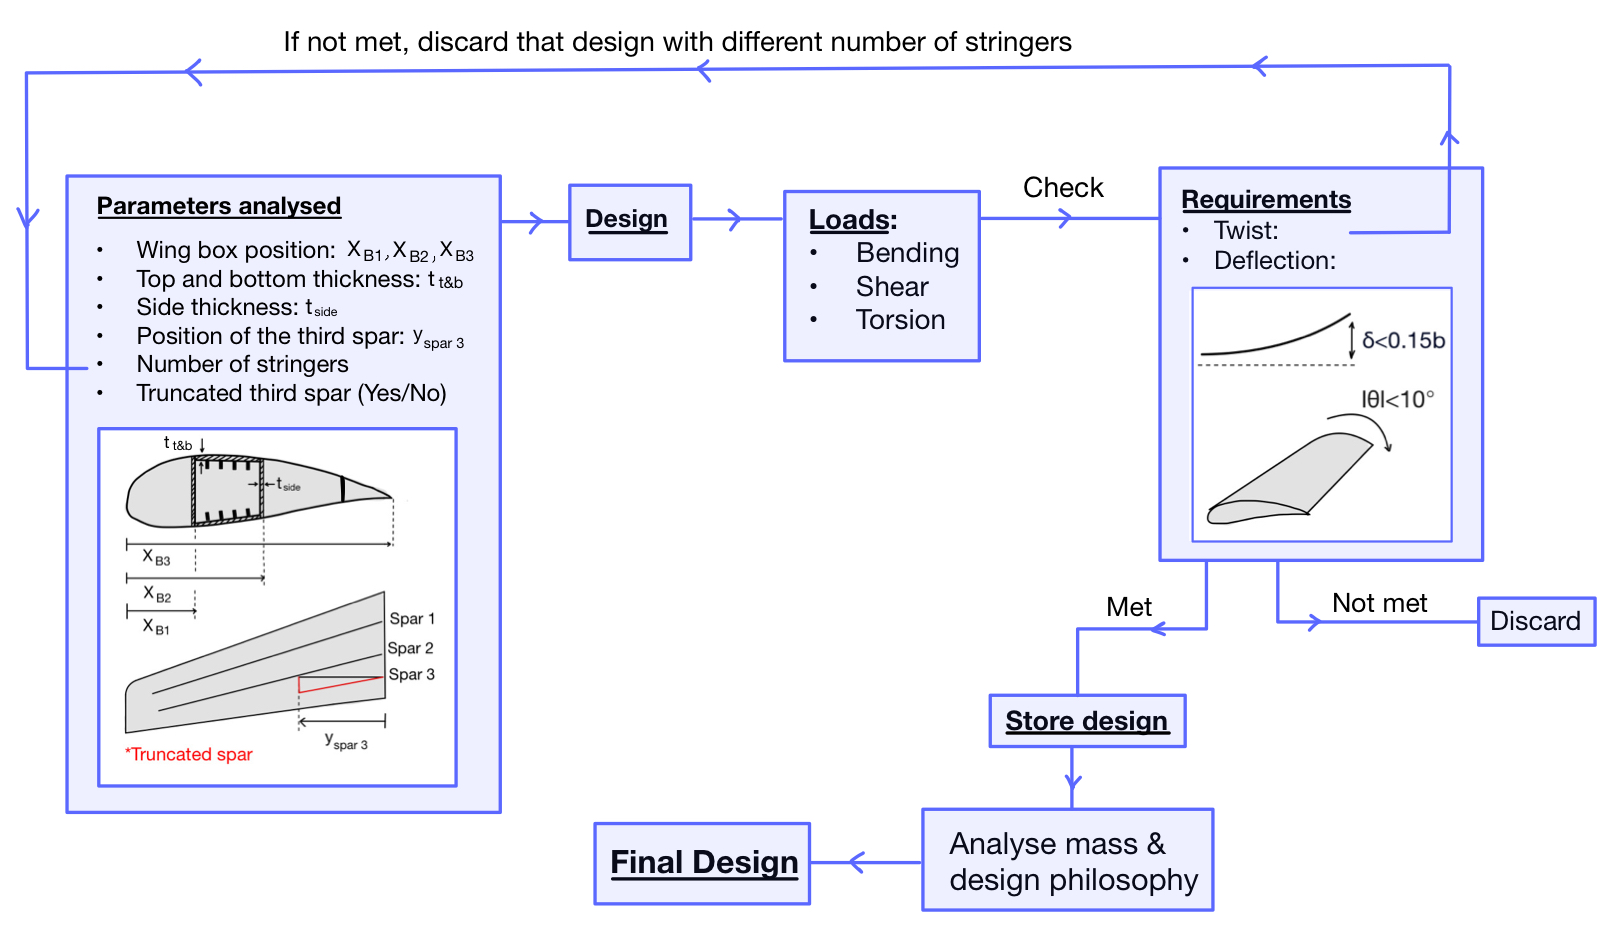
\includegraphics[width=1.1\linewidth]{figures/diagram python code.jpeg}
%     \caption{Production of designs procedure}
%     \label{fig:sketch_designs_procedure}
% \end{figure}



The code that was created for this step of the process takes several steps to calculate the final deflection and angle of twist. These are the two criteria that the wingbox design must perform sufficiently, the angle of twist cannot exceed 10$\degree$ and the deflection cannot exceed 15\% of the total span. \\

\noindent The code calculates through all the possible design points given by the set parameters. These parameters can be found in \ref{tab:design_parameters}.

\begin{table}[H]
    \caption{Design parameters used}
    \begin{tabular}{|c|c|c|}
        \hline
        \cellcolor{blue!15} Parameter & \cellcolor{blue!15} Range (step) & \cellcolor{blue!15} Note  \\
        \hline
        Chordwise position of the first spar & 0.2 - 0.45c (0.05c) & -\\
        \hline
        Chordwise position of the second spar & 0.25 - 0.6c (0.05c)  & starts 0.5 from first spar \\
        \hline
        Chordwise position of the third spar & 0.3 - 0.7c (0.05c) & starts 0.5 from second spar\\
        \hline
        Spanwise end of the third spar & 0.05 - 0.25b (0.025b) & \\
        \hline
        Transition to single cell wingbox & Truncated or merged  & \\
        \hline
        Thickness of the flanges of the wingbox & [0.5-2](0.1), [2-20](2) mm & Two ranges taken - one for low-thickness values and one for high\\
        \hline
        Thickness of shear webs of the wingbox & [0.5-2](0.1), [2-20](2) mm & Two ranges taken - one for low-thickness values and one for high. \\
        \hline
        Total number of stringers & 2 - 6 (2) & Divided for upper and lower spar cap\\
        \hline
    \end{tabular}
    \label{tab:design_parameters}
\end{table}

\noindent To do these calculations, the first thing needed is the geometry from these input parameters. This is done by taking the airfoil found in Wing Aerodynamic Design\cite{Koppejan2024WingDesign} and formatting it in such a way that with the chordwise position of the spars the main shape could be extrapolated. Afterwards, together with all the other parameters, the entire geometry of the wingbox is defined. From the geometry, the centroid together with its moment of inertia could be calculated for each spanwise position. This gave way to calculate the torsional stiffness as well as the tip deflection.\\

Seeing as the current parameters would calculate 86 billion different designs an additional metric needed to be introduced in order to screen through the results. For this reason a minimum weight criterion would be introduced. Having a minimum weight criterion restrains the design from being over-engineered, while still passing the requirements mentioned before. 



Format the airfoil geometry in such a way that the wingbox geometry can be extrapolated using the chordwise position of the spars.


    from this, we get the cross-sectional area of the wingbox at all spanwise points

    2. using the cross-section, get centroid, $I_{xx}$ and $I_{yy}$ 

\subsection{Torsional Stiffness}

Given that the wing will be experiencing torsional loads, the design should ensure that it can withstand those. The torsional stiffness determines Whether a wing box can or can not operate within that regime. The torsional stiffness,$TS$, is defined as the product of the torsional constant $J$ and the shear modulus $G$.(\autoref{eq: Torsional stiffness}\cite{})\todo{cite the eq from the SA book}

\begin{equation}
    \label{eq: Torsional stiffness}
    TS = J(z)\cdot G
\end{equation}

In \autoref{eq: Torsional stiffness} G is a constant, however, $J$ depends on the position with respect to the root chord, z. A function for calculating the torsional constant $J$ needs to be defined to determine how the stiffness changes throughout the wing. Computing the torsional constant is quite simple for a single-cell wing box, however, the computation for a multi-cell wingbox is a bit more tedious. Computing the torsional constant $J$ can be done by using \autoref{eq:single-cell}, where $A$ is the enclosed area of the wingbox and $t$ is the thickness which is integrated over the circumference.



\begin{equation}
J = \frac{4A^2}{\oint \frac{ds}{t}}
\label{eq:single-cell}
\end{equation}

For most aircraft, a single-cell wingbox is sufficient for withstanding the torsional loads, however, considering that the aircraft for which the wingbox is being designed is a large passenger aircraft, a multi-cell wingbox is used. A multi-cell wingbox ensures that the required stiffness is met and helps reduce spar buckling which will be analyzed in the future. Computing the torsional stiffness is done quite differently than from the single-cell case.  The approach is getting the constant from analyzing the shear flow,$q$, and the rate of torsion, $\frac{d\theta}{\dy}$ from which a system of three equations is solved. The first equation, \autoref{eq: Torque}, is obtained by applying a unit torque of 1 Nm. 

\begin{equation}
    T = 2\cdot A_1 \cdot q_1 + 2\cdot A_1 \cdot q_1 = 1
    \label{eq: Torque}
\end{equation}

$A_i$ is the enclosed area of each of the cells(1=left, 2=right) and $q_i$ is the shear flow. 

\begin{figure}
    \centering
    \includegraphics[width=0.5\linewidth]{}
    \caption{Caption}
    \label{fig:enter-label}
\end{figure}

\subsection{Tip deflection}

As one of the defining functional requirements, special considerations must be made to limit tip deflection. As the wing experiences bending and shear forces, it will experience accumulated deflection along the wing span. \\

\noindent After obtaining the bending moment, analyzed in \autoref{sec:fd_shear_moment_torque}, the slope of the wing as a function of the location of the span can be defined in \autoref{eq:wing_slope} \cite[p. 599]{Hibbeler2018MechanicsUnits}. 

\begin{equation} \label{eq:wing_slope}
    \frac{dv(x)}{dx} = - \frac{1}{E} \int_{x}^{b/2} \frac{M(x)}{I(x)} \cdot dx + C_1
\end{equation}

\noindent Here, $v(x)$ is the wing deflection, and $I(x)$ is the function of the moment of inertia along the wingspan, which shall vary for each iterated configuration. $C_1$ is the integration factor, and Young's modulus $E$ can be excluded from the integral, as it is a constant for the material used. \\


\noindent Integrating further, the wing deflection $v(x)$ can be defined as follows in \autoref{eq:wing_deflection}

\begin{equation} \label{eq:wing_deflection}
    v(x) = \int_{x}^{b/2} \left(\frac{dv(x)}{dx} + C_1 \right) \cdot dx + C_2
\end{equation}

\noindent Where $C_2$ represents the 2nd integration factor. \\

\noindent Due to the nature of the wingbox, it can be assumed to behave like a cantilevered beam. Thus, two initial conditions are enforced. Both the slope and deflection of the wing at the root must be equal to 0 due to it being an immovable support point. These characteristics determine the integration factors, where \autoref{eq:slope_0} determines $C_1$, and \autoref{eq:deflection_0} determines $C_2$:

\begin{equation} \label{eq:deflection_0}
    v(0) = 0
\end{equation}
\begin{equation} \label{eq:slope_0}
    \frac{dv(0)}{dx} = 0
\end{equation}

\noindent Ultimately, this double integral can be encoded in the Python code to iterate over in \autoref{sec:python_results} to verify if a configuration, with its accompanying moment of inertia $I$, meets the maximum deflection constraint defined earlier.


\section{Results of the Python code}
\label{sec:python_results}
To produce designs that meet the required specifications, the procedure shown in \autoref{fig:sketch_designs_procedure} was followed. This process needed to be iterated across every possible combination of the parameters that are being analyzed. The designs that meet both requirements will later be compared. The final choice will be made based on the mass of the design and the design philosophies.

\begin{figure}[H]
    \centering
    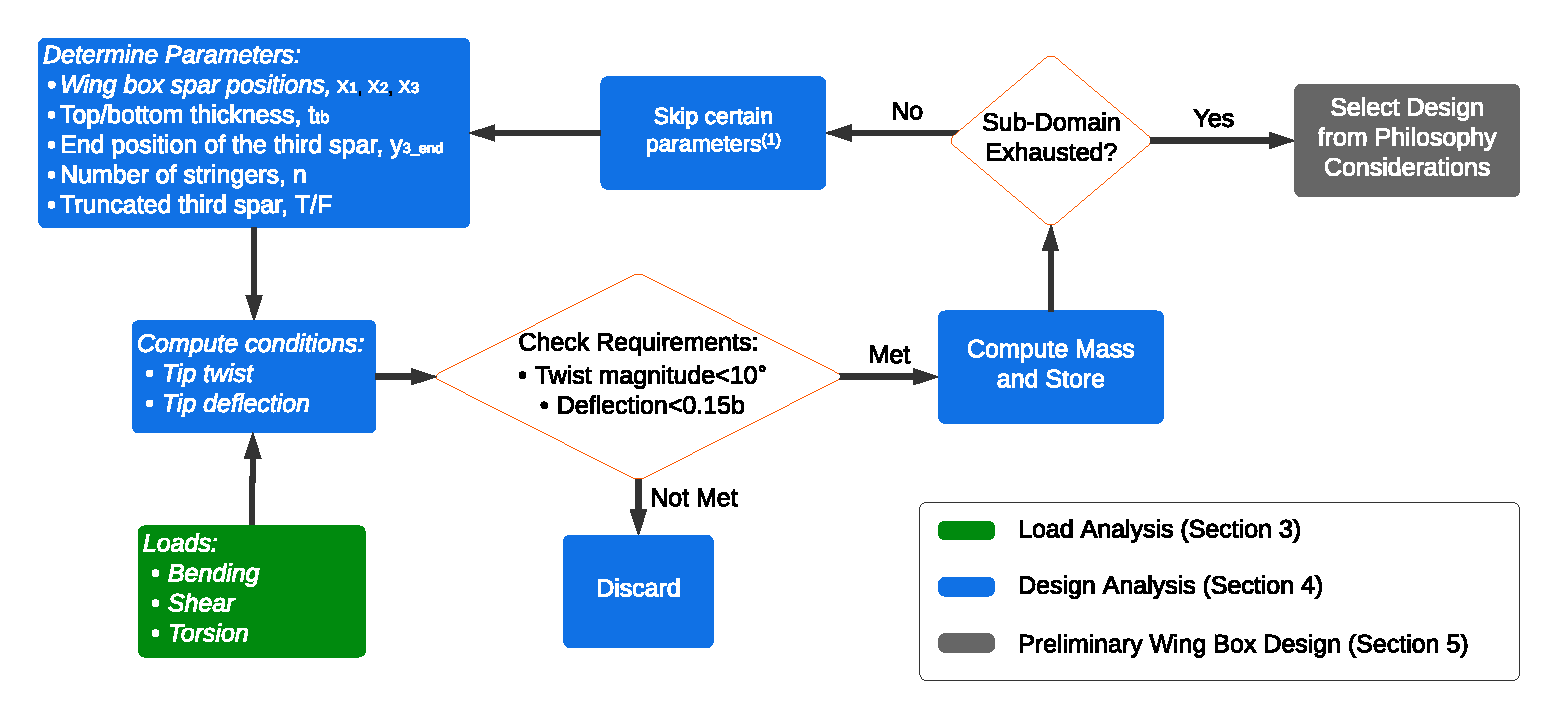
\includegraphics[width=\linewidth]{figures/Flowchart_Iteration.pdf}
    \caption{Production of designs procedure}
    \label{fig:sketch_designs_procedure}
\end{figure}